\documentclass{beamer}
\usetheme{COURS}
\usepackage{tcolorbox}
\usepackage{textpos}
\usetikzlibrary{arrows,automata}
\usepackage{minted}
\usemintedstyle{emacs}


\def\red{\color{red}}
\def\blue{\color{blue}}
\def\green{\color{green}}

\def\opstyle#1{\ensuremath{\operatorname{#1}}}

\title[High Performance Combinatorics]%
{\bf High Performance Combinatorics}
\author{\textbf{\Large Florent Hivert}\\[5mm]
  Mél : \texttt{Florent.Hivert@lri.fr}\\
  Adresse universelle : \texttt{http://www.lri.fr/\~{ }hivert}
}
\date{}

\begin{document}
\newcommand{\Count}{\opstyle{count}}
\newcommand{\List}{\opstyle{list}}
\newcommand{\Iter}{\opstyle{iter}}
\newcommand{\Unrank}{\opstyle{unrank}}
\newcommand{\Rank}{\opstyle{rank}}
\newcommand{\First}{\opstyle{first}}
\newcommand{\Next}{\opstyle{next}}
\newcommand{\Random}{\opstyle{random}}

\newcommand{\Concat}{\opstyle{concat}}
\newcommand{\BS}{\opstyle{BitString}}
\newcommand{\Perm}{\opstyle{Perm}}
\newcommand{\Union}{\opstyle{Union}}
\newcommand{\Prod}{\opstyle{Prod}}

\newcommand{\Pos}{\opstyle{Pos}}
\newcommand{\Bin}{\opstyle{Bin}}
\newcommand{\Gray}{\opstyle{Gray}}

\newcommand{\mA}{\mathcal{A}}
\newcommand{\mB}{\mathcal{B}}
\newcommand{\mC}{\mathcal{C}}
\newcommand{\mD}{\mathcal{D}}
\newcommand{\mE}{\mathcal{E}}
\newcommand{\mI}{\mathcal{I}}
\newcommand{\mZ}{\mathcal{Z}}

\newcommand{\Oh}{O}

%***********************************************************************
\frame{\titlepage}
%***********************************************************************

\begin{frame}{Instruction vectorielles entières}

  Registre: \texttt{epi8,epu8}: 128~bits $=$ 16~octets
  \bigskip

  Encore plus: AVX, AVX2, AVX512
  \medskip

  \begin{itemize}
  \item Opérations Arithmetiques/logiques: \texttt{and, or, add, sub, min, max, abs, cmp}
  \item Recherche de bits: \texttt{popcount}, \texttt{bfsd}
  \end{itemize}
  \pause
  Encore plus intéressant pour nous:
  \begin{itemize}
  \item Manipulation de tableau: \texttt{blend, broadcast, shuffle}
  \item Comparaison de chaînes de caractères: \texttt{cmpistr} (lex, find).
  \end{itemize}
  \begin{tcolorbox}
    \centering
    \textbf{\large Manipulations très efficaces !}
  \end{tcolorbox}
\end{frame}

\begin{frame}{Exemple: les réseaux de tris}

  Knuth AoCP3 Fig.~51 p.~229:
  \[
  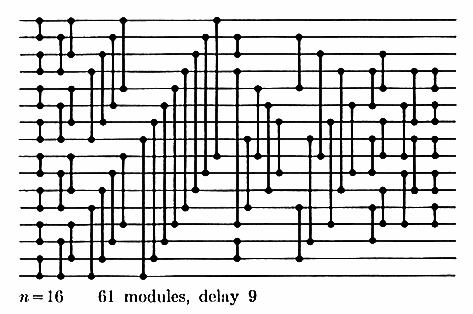
\includegraphics[height=5cm,width=11cm]{media/nibble-sort.png}
  \]
\end{frame}
\begin{frame}[fragile]

\small
\begin{minted}{C++}
// Sorting network Knuth AoCP3 Fig. 51 p 229.
static const array<perm, 9> rounds = {{
       { 1, 0, 3, 2, 5, 4, 7, 6, 9, 8,11,10,13,12,15,14},
       { 2, 3, 0, 1, 6, 7, 4, 5,10,11, 8, 9,14,15,12,13},
       ...
    }};
\end{minted}
\begin{minted}{C++}
perm sort(perm a) {
  for (perm round : rounds) {
    perm minab, maxab, mask;
    perm b = _mm_shuffle_epi8(a, round);
    mask = _mm_cmplt_epi8(round, permid);
    minab = _mm_min_epi8(a, b);
    maxab = _mm_max_epi8(a, b);
    a = _mm_blendv_epi8(minab, maxab, mask);
  }
  return a;
}
\end{minted}
\end{frame}

\end{document}
